% vim:autoindent:set textwidth=78:

\section{Lavorare con le proiezioni}\label{label_projections}
\index{proiezioni!lavorare con}

% when the revision of a section has been finalized, 
% comment out the following line:
%\updatedisclaimer

QGIS consente all'utente di definire un CRS (Coordinate
Reference System) globale o per ogni singolo progetto per i layer privi di un
CRS predefinito. Consente inoltre di definire sistemi di coordinate
personalizzati e supporta la riproiezione al volo (on-the-fly, OTF) dei layer
vettoriali. Tutte queste caratteristiche permettono all'utente di visualizzare
contemporaneamente layer con diversi CRS correttamente sovrapposti.

\subsection{Panoramica del supporto alle proiezioni}\label{label_projoverview}

QGIS supporta all'incirca 2.700 CRS noti. Le definizioni di ognuno di questi
CRS sono immagazzinate in un database SQLite che viene installato con QGIS.
Normalmente non è necessario manipolare il database direttamente, in effetti
tale operazione può causare il malfunzionamento del supporto alla proiezione.
I CRS personalizzati sono salvati in un database utente.
Si veda la sezione \ref{sec:customprojections} per informazioni
sulla gestione dei CRS personalizzati.

I CRS disponibili in QGIS sono basati su quelli definiti da EPSG\index{EPSG}
e sono largamente ispirati alle tabelle spatial\_references
di PostGIS\index{PostGIS} versione 1.x. Gli identificatori EPSG sono presenti
nel database e possono essere usati per richiamare e definire i CRS in QGIS.

Per usare la proiezione al volo (OTF), i dati devono contenere informazioni
sul proprio sistema di coordinate oppure bisogna definire un CRS per il layer,
per il progetto oppure globale.
Per layer PostGIS QGIS usa l'identificatore dello spatial reference
specificato quando il layer è stato creato. Per i dati supportati da OGR,
QGIS fa affidamento sulla presenza di un file con formato caratteristico che
definisce il CRS. Per gli shapefile, questo significa avere l'indicazione del
CRS in formato Well Known Text (WKT)\index{WKT}. Il file della proiezione
ha lo stesso nome dello shapefile ma ha estensione prj. Per esempio uno
shapefile chiamato \filename{alaska.shp} avrà un corrispondente file di
proiezione chiamato \filename{alaska.prj}.

\subsection{Specificare una proiezione}
\index{proiezioni!specifiche}
\label{sec:projection-specifying}

QGIS non imposta più il CRS della mappa al sistema di coordinate per primo
layer caricato. Quando si avvia una sessione QGIS con layer privi di CRS,
è necessario controllare e definire il CRS di questi layer. Questo può
essere fatto globalmente o per ogni progetto nella scheda \tab{CRS} sotto
la voce di menu \mainmenuopt{Impostazioni} >
\dropmenuopttwo{mActionOptions}{Opzioni} (Si veda la Figura~\ref{fig:crsdialog}). 

\begin{itemize}
\item \checkbox{Richiesta per CRS} 
\item \checkbox{CRS predefinito utilizzato dal progetto}
\item \checkbox{Verrà utilizzato il seguente CRS globale predefinito
visualizzato qui sotto}
\end{itemize}

In QGIS il CRS globale predefinito è \texttt{proj=longlat +ellps=WGS84 +datum=WGS84
+no\_defs} ma può essere cambiato, la nuova impostazione verrà salvata per le
successive sessioni.

\begin{figure}[ht]
   \begin{center}
   \caption{Scheda CRS nella finestra opzioni di QGIS \nixcaption}\label{fig:crsdialog}\smallskip
   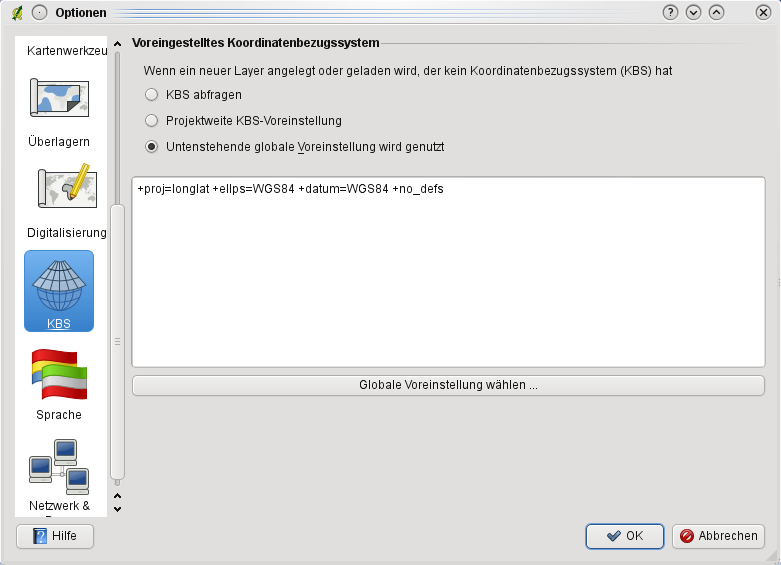
\includegraphics[clip=true, width=12cm]{crsdialog}
\end{center}
\end{figure}

Per definire il CRS di un layer privo di tale informazione, si può anche agire
nella scheda \tab{Generale} della finestra delle proprietà raster (\ref{label_generaltab})
e delle proprietà vettore (\ref{vectorgeneraltab}). Se il CRS è già stato
definito, verrà mostrato come nella figura~\ref{fig:vector_symbology}.

\subsection{Definire la proiezione al volo (OTF)}\label{label_projstart}

In QGIS la proiezione al volo (OTF) non è abilitata di default, tale funzione
è attualmente supportata solo per layer vettoriali. Per usare la proiezione OTF,
bisogna aprire la finestra di dialogo
\dropmenuopttwo{mActionOptions}{Proprietà progetto}, selezionare un CRS
e attivare la casella di controllo \checkbox{Abilita la "modifica al volo"
della trasformazione CRS}.
Ci sono due modi per aprire questa finestra:

\begin{enumerate}
\item Selezionare \dropmenuopttwo{mActionOptions}{Proprietà progetto} dal menu
\mainmenuopt{Impostazioni}.
\item Cliccare sull'icona \toolbtntwo{mIconProjectionEnabled}{Stato CRS}
nell'angolo destro della barra di stato.
\end{enumerate}

Se è già stato caricato un layer, e si vuole abilitare la proiezione OTF, è
buona norma aprire la scheda \tab{Sistema di coordinate di riferimento
spaziale (CRS)} della finestra di dialogo \dialog{Proprietà progetto} e
individuare nell'elenco il CRS attualmente impostato, quindi attivare
la casella di controllo \checkbox{Abilita la "modifica al volo"
della trasformazione CRS}. Ogni layer caricato successivamente sarà quindi
riproiettato al volo nel CRS definito.

La sched \tab{Sistema di coordinate di riferimento
spaziale (CRS)} della finestra \dialog{Proprietà progetto}
contiene quattro importanti componenti come individuate nella Figura \ref{fig:projections}
e di seguito descritte.

\begin{figure}[ht]
   \begin{center}
   \caption{Finestra di dialogo per l'impostazione della proiezione \nixcaption}\label{fig:projections}\smallskip
   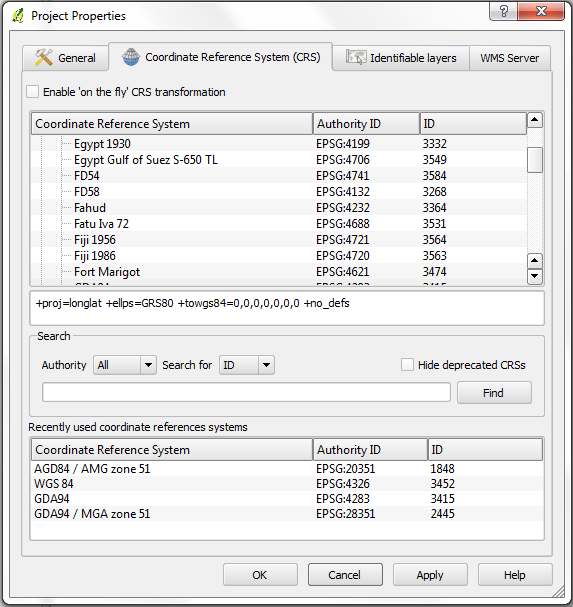
\includegraphics[clip=true, width=12cm]{projectionDialog}
\end{center}  
\end{figure}

\begin{enumerate}
\item \textbf{Abilita la "modifica al volo" della trasformazione CRS}\index{proiezioni!abilitare} -
questa casella di controllo è usata per abilitare o disabilitare la proiezione
OTF. Quando è deselezionata, ogni layer è tracciato usando le coordinate lette
dal dato sorgente. Se abilitata, le coordinate di ogni layer sono riproiettate
verso il sistema di coordinate definito per la mappa.
\item \textbf{Coordinate del Sistema di Riferimento} - è la lista di tutti i CRS
supportati da QGIS, inclusi i sitemi di coordinate geografiche, piane e
quelli personalizzati. Per usare un CRS, selezionarlo dalla lista espandendo
la voce appropriata. Il CRS attivo è preselezionato.
\item \textbf{Stringa Proj4} - è la stringa CRS usata dal motore per le
proiezioni the Proj4. È un testo in sola lettura a solo scopo informativo.
\item \textbf{Trova} - se si conosce l'identificatore EPSG o il nome del CRS
che si vuole impostare, può essere usata questa area di ricerca per trovarlo
nell'elenco inserendo l'identificatore e cliccando su \button{Trova}.
\end{enumerate}

\begin{Tip}
 \caption{\textsc{Finestra delle proprietà della proiezione}}
\qgistip{
Se si apre la finestra \dialog{Proprietà progetto} dal menu
\mainmenuopt{Impostazioni}, bisogna cliccare sulla scheda \tab{Sistema di coordinate di riferimento
spaziale (CRS)} per vedere le impostazioni del CRS. Aprendo la finestra
dall'icona \toolbtntwo{mIconProjectionEnabled}{Stato CRS} verrà portata invece
immediatamente in primo piano la scheda \tab{Sistema di coordinate di riferimento
spaziale (CRS)}.
}
\end{Tip}

\subsection{Proiezione definita dall'utente}\label{sec:customprojections}
\index{proiezione!personalizzare}

Se in QGIS non si trova la proiezione di cui si necessita, è possibile
definire un CRS personalizzato. Per fare ciò, selezionare
\dropmenuopttwo{mIconNew}{CRS personalizzato} dal menu
\mainmenuopt{Impostazioni}. I CRS personalizzati sono salvati nel database
utente di QGIS. Oltre ai CRS personalizzati, questo database contiene anche i
segnalibri geospaziali e altri dati personalizzati. 

\begin{figure}[ht]
   \begin{center}
   \caption{Finestra del CRS personalizzato \nixcaption}\label{fig:customprojections}\smallskip
   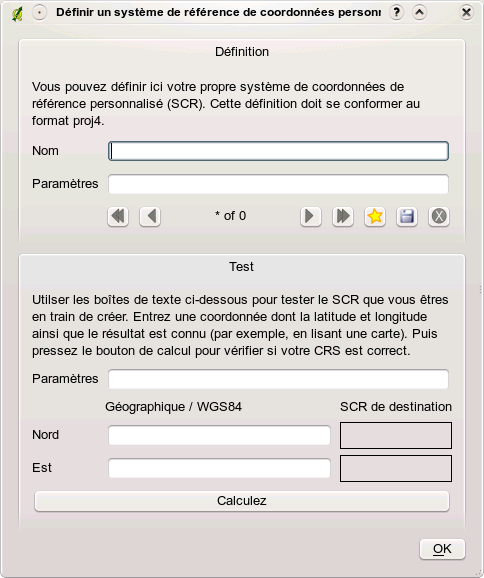
\includegraphics[clip=true, width=12cm]{customProjectionDialog}
\end{center}  
\end{figure}

La definizione di un CRS personalizzato in QGIS richiede una buona
comprensione delle librerie Proj.4. Per iniziare, fare riferimento al
documento Cartographic Projection Procedures for the UNIX Environment - A User's Manual
by Gerald I. Evenden, U.S. Geological Survey Open-File Report 90-284, 1990
(disponibile all'indirizzo \url{ftp://ftp.remotesensing.org/proj/OF90-284.pdf}).
Questo manuale descrive l'uso di \usertext{proj.4} e delle relative utilità da
riga di comando. I parametri cartografici usati da \usertext{proj.4} sono
descritti nel manuale utente e sono identici a quelli usati da QGIS. 

La finestra \dialog{Definizione Sistema Riferimento Spaziale Personalizzato}
richiede solo due parametri per definire un CRS personalizzato: 
\begin{enumerate}
\item un nome descrittivo e
\item i parametri cartografici in formato PROJ.4.
\end{enumerate}
Per creare un nuovo CRS, cliccare il pulsante \toolbtntwo{mIconNew}{Nuovo} e
inserire il nome descrittivo e i parametri CRS. Successivamente salvare il CRS
cliccando sul pulsante \toolbtntwo{mActionFileSave}{Salva}.

Si noti che la voce \guilabel{Parametri} deve iniziare con un blocco \usertext{+proj=},
per rappresentare il nuovo CRS.

È possibile testare i parametri CRS per vedere se danno risultati validi
cliccando sul pulsante \button{Calcola} nella sezione \guiheading{Prova} dopo
aver incollato i parametri CRS personalizzati nel campo \guilabel{Parameters}.
Inserire valori di latitudine e longitudine WGS 84 nei campi \guilabel{Nord} e
\guilabel{Est} rispettivamente. 
Cliccare su \button{Calcola} e confrontare i risultati con i valori noti nel
sistema CRS personalizzato. 

